% \begin{figure*}[!t]
% \centering
%   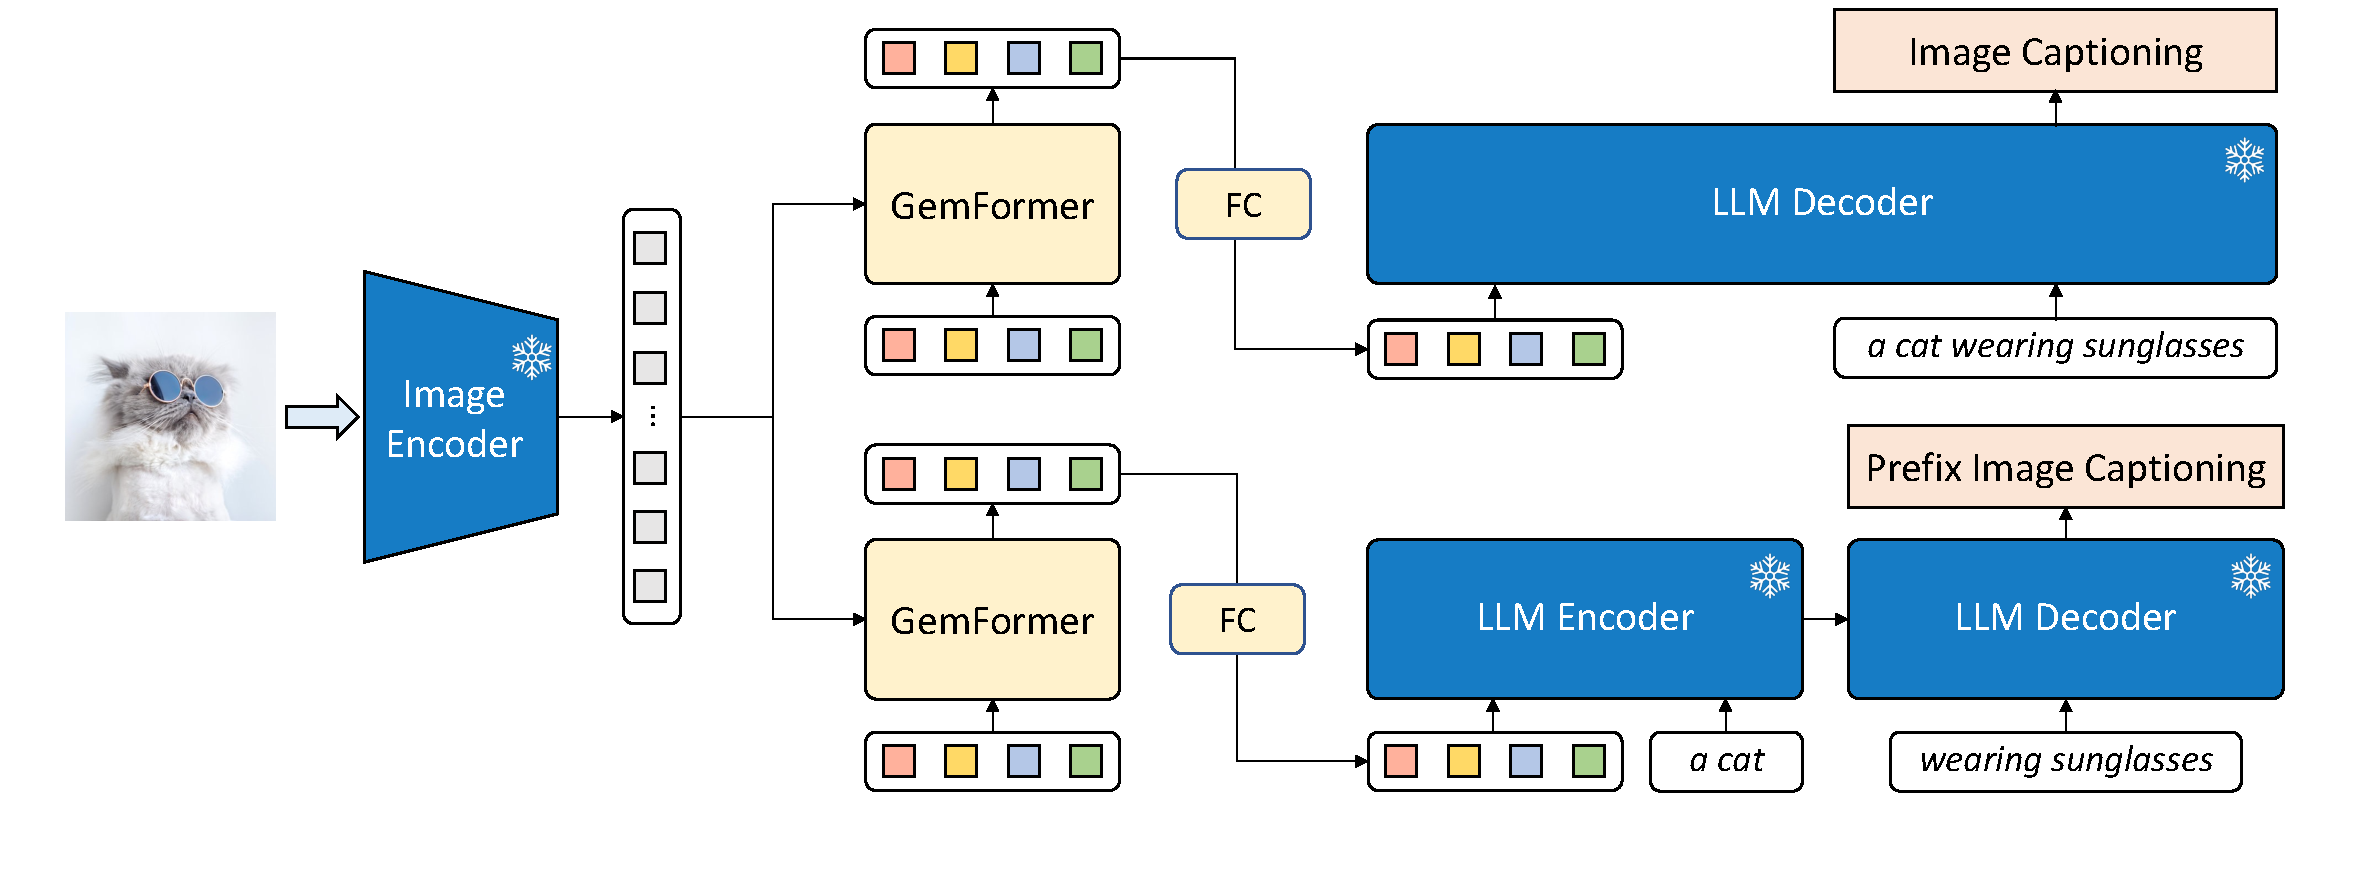
\includegraphics[width=\textwidth]{image/stage2.pdf}
% \vspace{-2ex}
% \caption{Pre-training.
% }
% %\vspace{-1ex}
% \label{fig:stage2}
% \end{figure*}

% \begin{figure*}[!t]
% \centering
%   
\includegraphics[width=\textwidth]{BLIPv2/image/fig3.pdf}
% \vspace{-2ex}
% \caption{Pre-training.}
% %\vspace{-1ex}
% \label{fig:stage2}
% \end{figure*}


\begin{figure*}[!t]
\centering
%   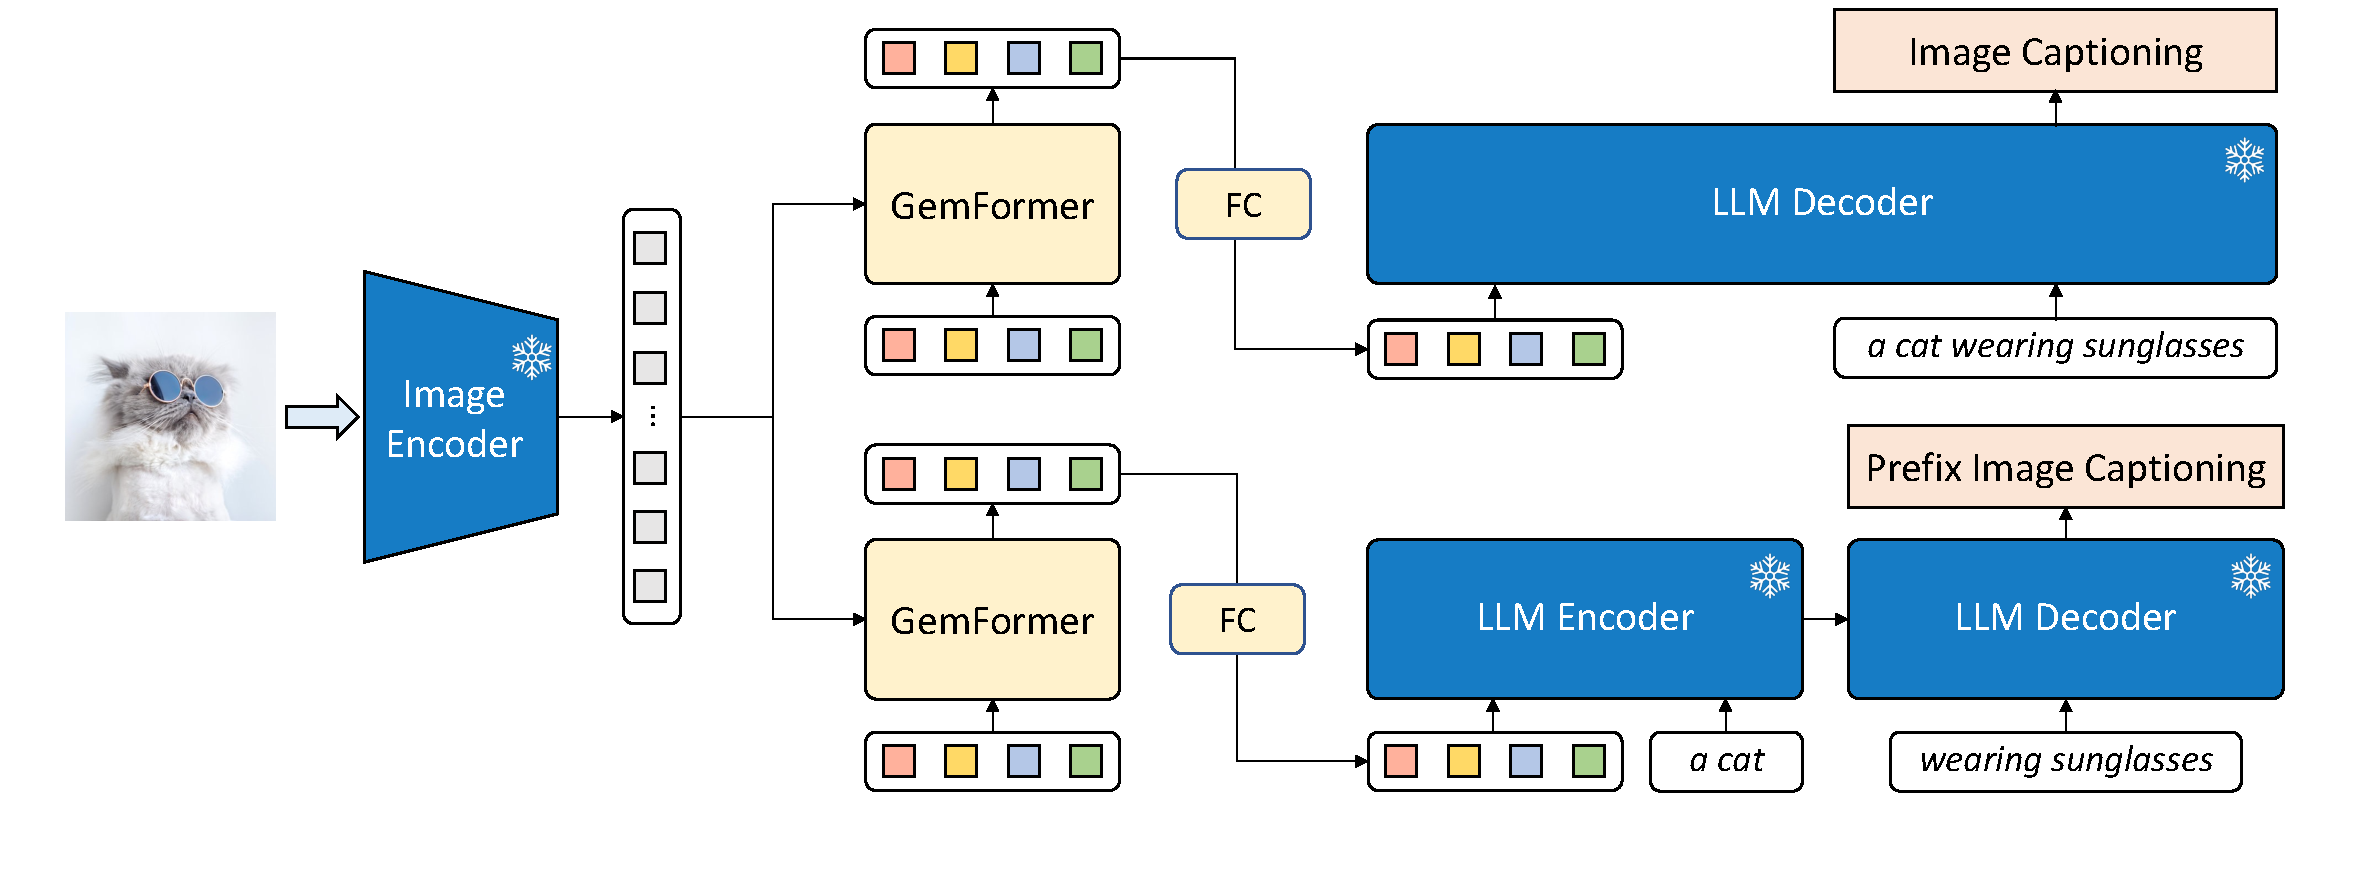
\includegraphics[width=\textwidth]{image/stage2.pdf}
  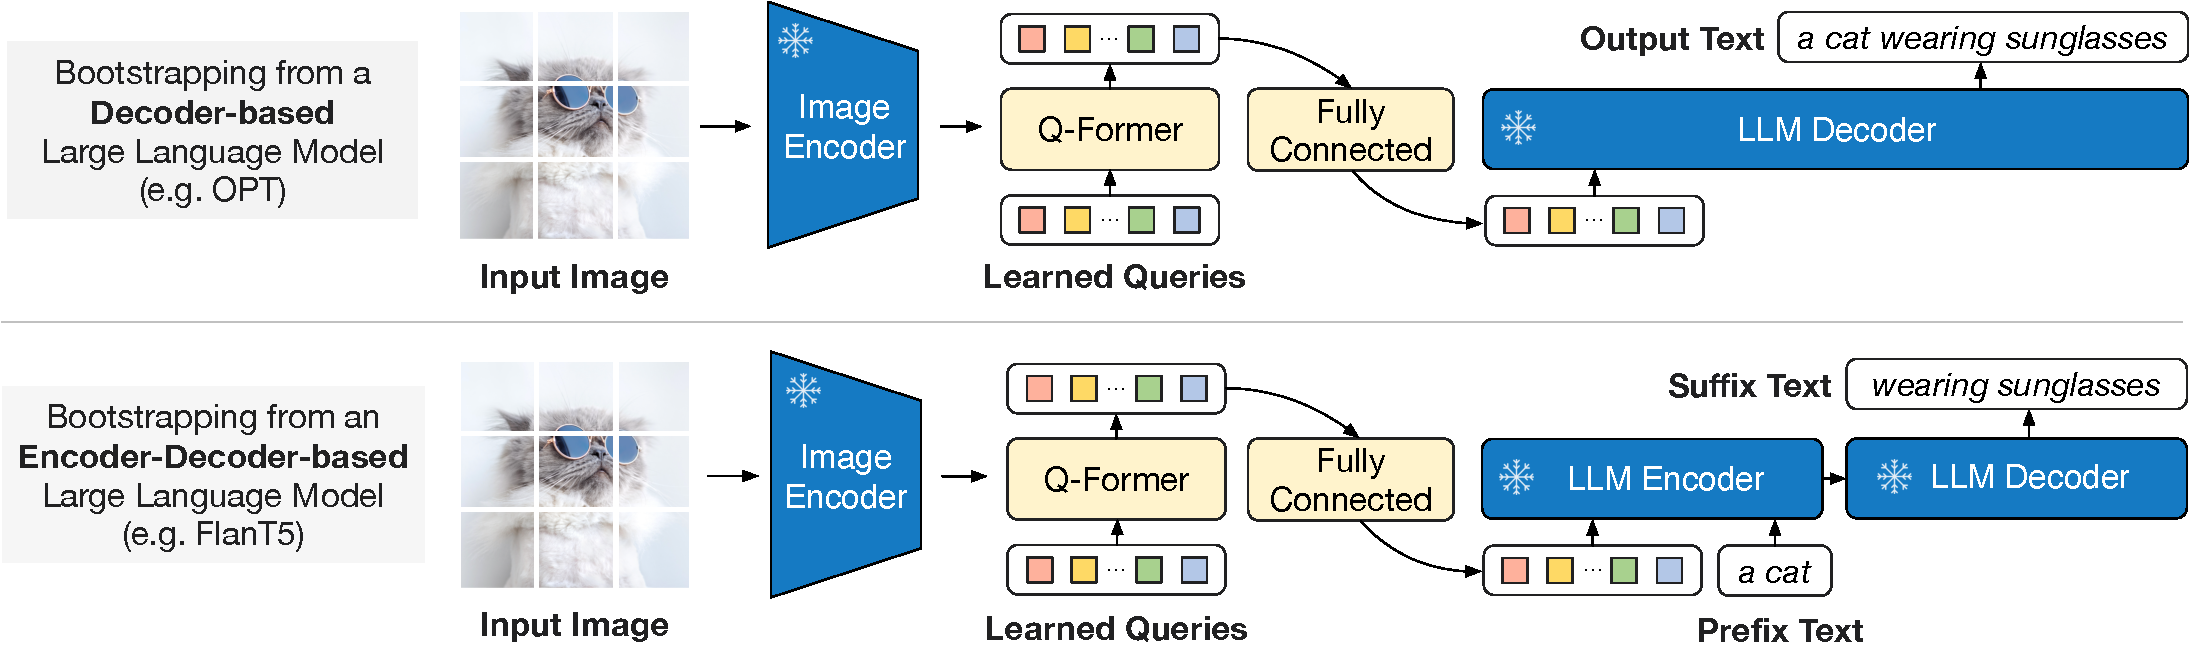
\includegraphics[width=0.9\textwidth]{image/fig3-v3.pdf}
\vspace{-2ex}
\caption{BLIP-2's second-stage vision-to-language generative pre-training, which bootstraps from frozen large language models (LLMs). (\textbf{Top}) Bootstrapping a decoder-based LLM (e.g. OPT). (\textbf{Bottom}) Bootstrapping an encoder-decoder-based LLM (e.g. FlanT5). The fully-connected layer adapts from the output dimension of the Q-Former to the input dimension of the chosen LLM.}
\vspace{-1.5ex}
\label{fig:stage2}
\end{figure*}

% \begin{figure*}[!t]
% \centering
% %   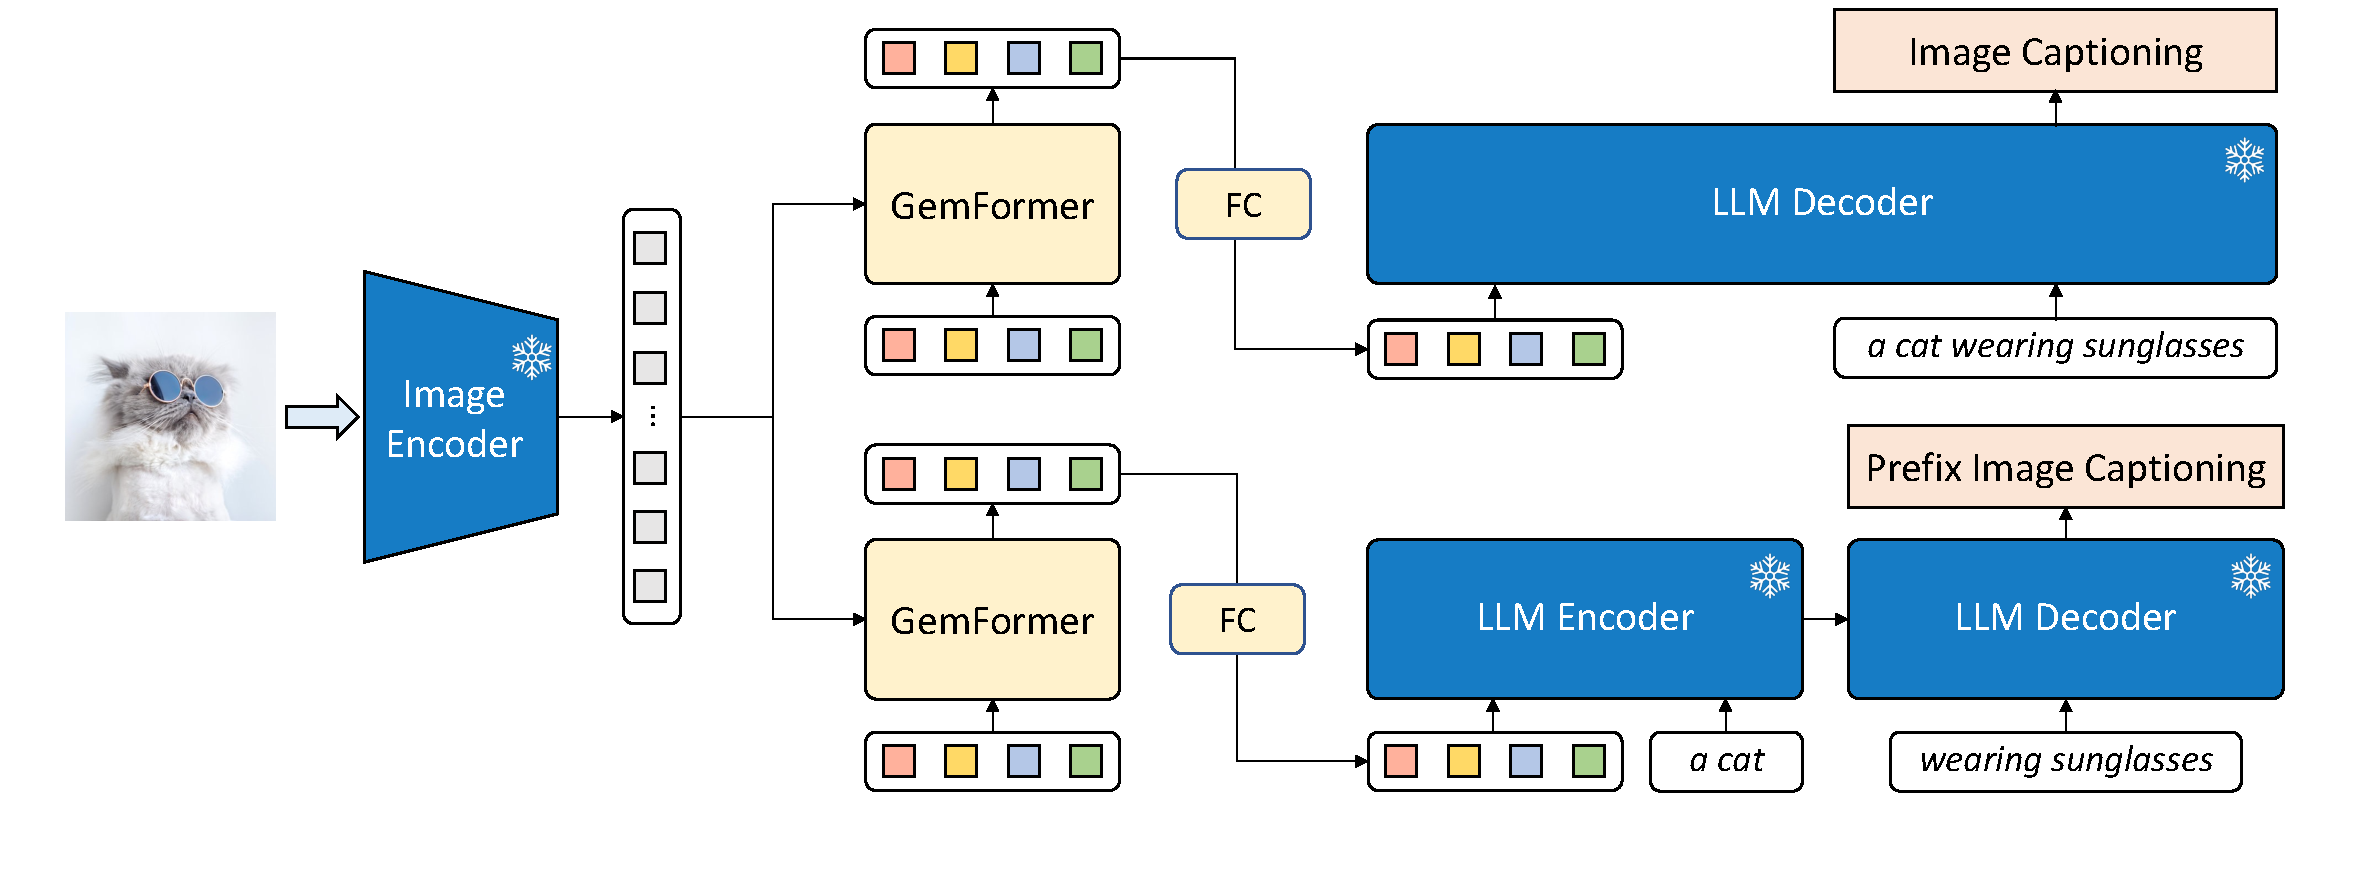
\includegraphics[width=\textwidth]{image/stage2.pdf}
%   
\includegraphics[width=0.8\textwidth]{BLIPv2/image/fig3-v2.pdf}
% \vspace{-2ex}
% \caption{Model architecture to bootstrap from frozen large language models (LLMs) with Q-Former. (\textbf{Top}) Bootstrapping a Decoder-based Large Language Model (e.g. OPT). (\textbf{Bottom}) Bootstrapping an Encoder-Decoder-based Large Language Model (e.g. FlanT5). The fully-connected layer adapts from the hidden dimension of the Q-Former to that of the chosen LLM.}
% %\vspace{-1ex}
% \label{fig:stage2}
% \end{figure*}



% \begin{figure*}[!t]
% \centering
% %   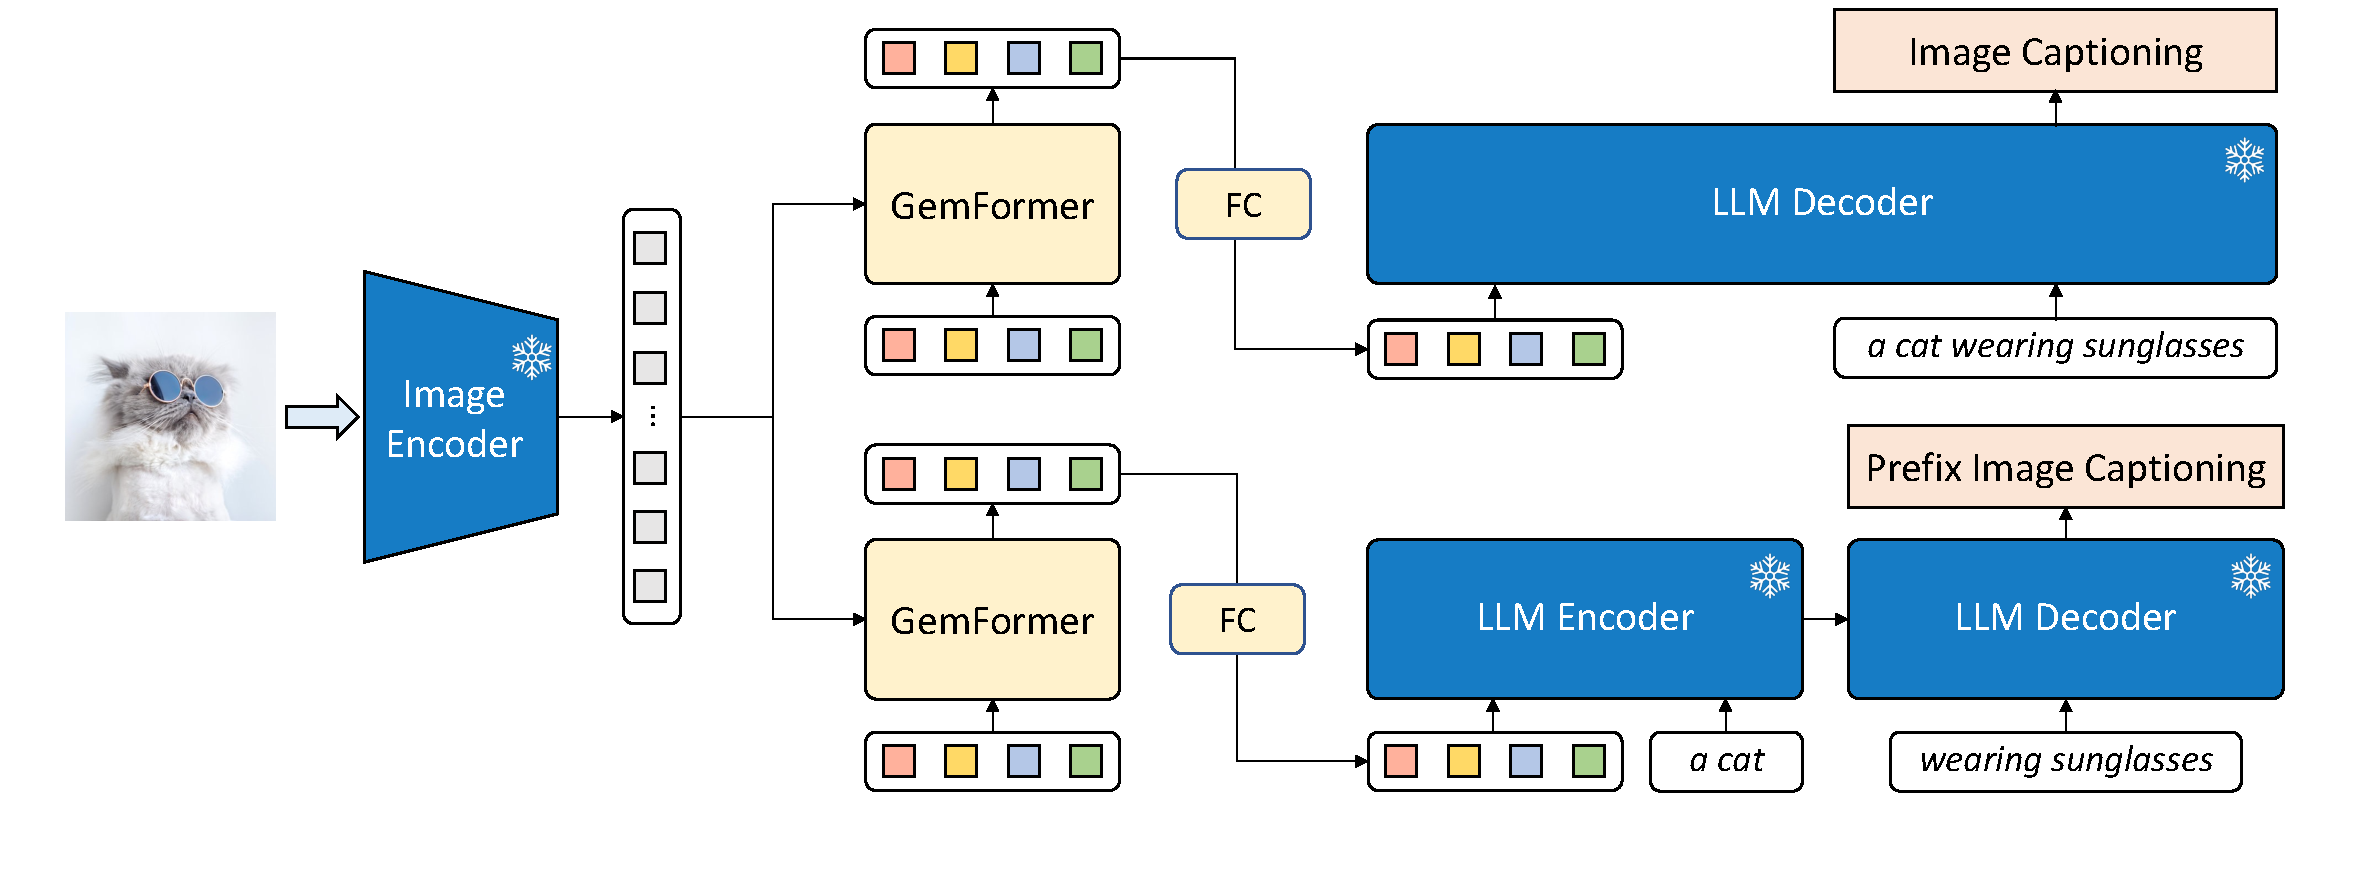
\includegraphics[width=\textwidth]{image/stage2.pdf}
%   
\includegraphics[width=0.8\textwidth]{BLIPv2/image/fig3-v2.pdf}
% \vspace{-2ex}
% \caption{Model architecture to bootstrap from frozen large language models (LLMs) with Q-Former. (\textbf{Top}) Bootstrapping a Decoder-based Large Language Model (e.g. OPT). (\textbf{Bottom}) Bootstrapping an Encoder-Decoder-based Large Language Model (e.g. FlanT5). The fully-connected layer adapts from hidden dimension in Q-Former to that of the chosen LLM.}
% %\vspace{-1ex}
% \label{fig:stage2}
% \end{figure*}